\chapter{Heap, Stack und die UML}

% **************************** Define Graphics Path **************************
\ifpdf
    \DeclareGraphicsRule{*}{mps}{*}{}
	\graphicspath{{Chapter3/Figs/UML/}{Chapter3/Figs/Raster/}{Chapter3/Figs/PDF/}{Chapter3/Figs/}}
\else
    \graphicspath{{Chapter3/Figs/UML/}{Chapter3/Figs/Vector/}{Chapter3/Figs/}}
\fi

In diesem Abschnitt werden noch einige weitere Themen behandelt, die prüfungsrelevant sind. Diese Themen werden lediglich angeschnitten und sollen einen Überblick geben. Die hier aufgeschriebenen Themen bestehen hauptsächlich aus den in den Tutorien übermittelteln Inhalten, da diese einen besseren Überblick vermittelten, als der in der Vorlesung vermittelte Stoff. Das kann auch der Grund für kleinere Abweichungen sein. Ich hoffe dennoch, dass die hier dargestellten Verfahren eine gute Übersicht geben können. 


\section{Heap und Stack}

In Java gibt es zwei Speicherbereiche, den \texttt{Stack} (dieser wurde in der Vorlesung auch als \texttt{Laufzeitkeller} bezeichnet) und den \texttt{Heap}. 

Der Stack speichert Methoden, Variablen und Parameter und funktioniert nach dem \texttt{LIFO} Prinzip (Last in First out). Das kann man sich wie eine Pringels Packung vorstellen. Man kann immer nur auf das oberste Element zugreifen, wenn dieses abgearbeitet wurde, kann man dann auf das darunter Liegende zugreifen usw.

Den Heap kann man sich als Wolke vorstellen, in dem die Objekte gespeichert werden. Dabei wird von der JVM (Java Virtual Machine) dafür gesorgt, dass genug Platz für die Objekte reserviert wird. Dieser Platz wird beispielsweise für Instanzvariablen benötigt. An dieser Stelle ist es wichtig, dass man versteht, dass diese Instanzvariablen nicht auf dem Stack leben, sondern im Objekt, welches auf dem Heap liegt. Für int-Literale werden 32 Bit Speicherplatz beansprucht, für long und double Werte 64 Bit, diese sind jedoch als Einheit zu betrachten, werden also nicht aufgeteilt in 2 $\cdot$ 32 Bit.

Eine Besonderheit ist, wenn eine dieser Instanzvariablen ein weiteres Objekt ist. Stellen wir uns eine Klasse \texttt{Person} vor, die als Instanzvariable einen Ehepartner vom Typ \texttt{Person} hat. Dann macht Java nicht in dem eigentlichen Objekt Platz für den Ehepartner, sondern initialisiert ein komplett neues Objekt vom Typ Person, und speichert in dem ursprünglichen Objekt eine Referenz (auch als \texttt{Zeiger} oder \texttt{Pointer} bezeichnet) zu dem neu erstellten Objekt.

Das alles hört sich jetzt erst mal sehr komplex an, deswegen macht es Sinn, wenn man sich das Ganze mal anhand eines Beispiels anguckt. Dies wollen wir anhand des folgenden Codes machen:

\begin{lstlisting}
Person meier;
Person mueller;

meier = new Person();
meier.alter = 74;
meier.nachname = "Meier";

mueller = new Person();
mueller.alter = 22;
mueller.nachname = "Müller";
\end{lstlisting}

Wenn wir die letzte Zeile des obigen Code-Beispiels durchlaufen, sehen Stack (links) und Heap (rechts) wie folgt aus. Die kryptische Bezeichnung 0x123 soll lediglich heißen, dass hier eine Adresse gespeichert wird, die auf das Objekt zeigt. Es handelt sich hierbei um eine Beispieladresse, da Objekte dynamisch allokiert wird (also der Speicher reserviert wird).

\begin{figure}[htbp!] 
\centering    
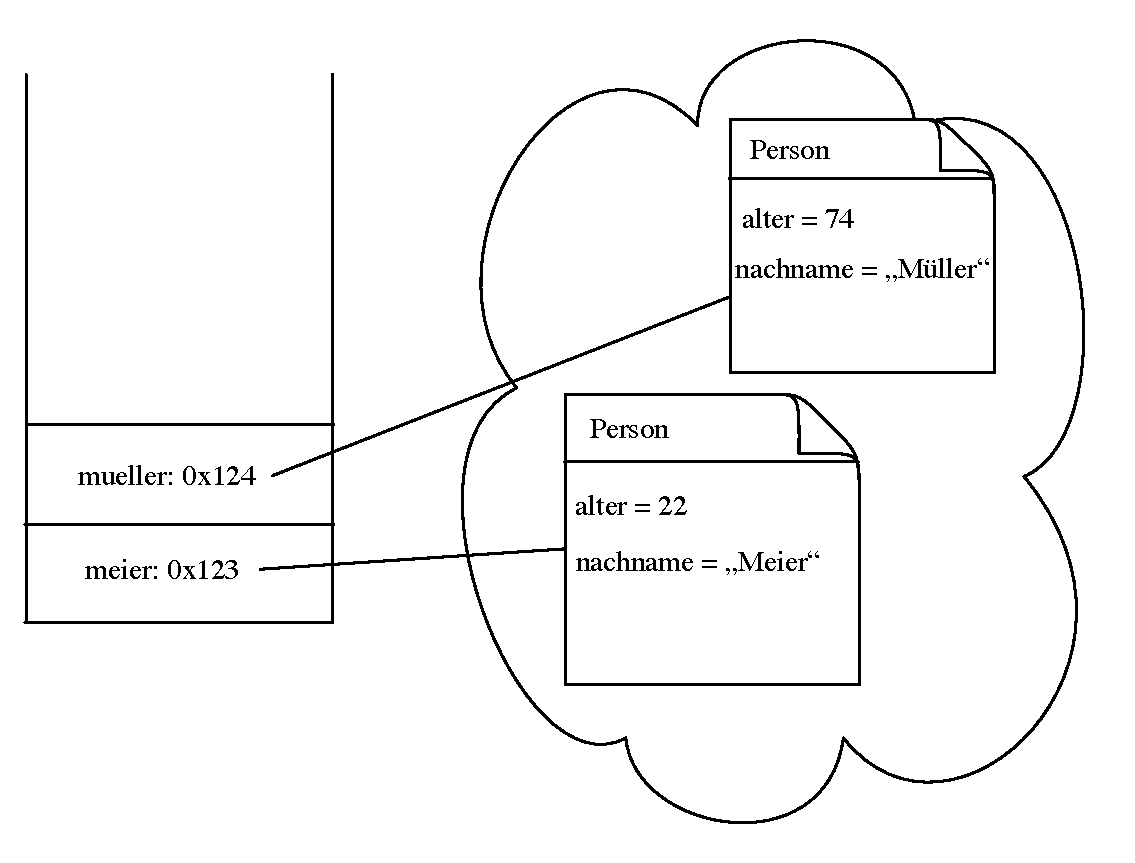
\includegraphics[width=0.8\textwidth]{stackheap_1}
\label{fig:stackheap1}
\caption{Die Adresse der zwei Objekte liegt auf dem Stack, die zwei Objekte liegen jedoch auf dem Heap.}
\end{figure}

Nun wollen wir das oben angesprochene Konzept erweitern, indem wir die beiden Personen heiraten lassen. Hierzu fügen wir die Funktion \texttt{heiraten(Person person)} auf.

\begin{lstlisting}
Person mueller;

meier = new Person();
meier.alter = 74;
meier.nachname = "Meier";

mueller = new Person();
mueller.alter = 22;
mueller.nachname = "Müller";

meier.heiraten(mueller);
\end{lstlisting}

Durch die Methode heiraten, wird die Adresse des ehepartners in der Variable Ehepartner gespeichert. Diese Adresse zeigt auf das Objekt des ehepartners. Da beide Personen miteinander verheiratet sind, zeigen sie jeweils aufeinander.

\begin{figure}[htbp!] 
\centering    
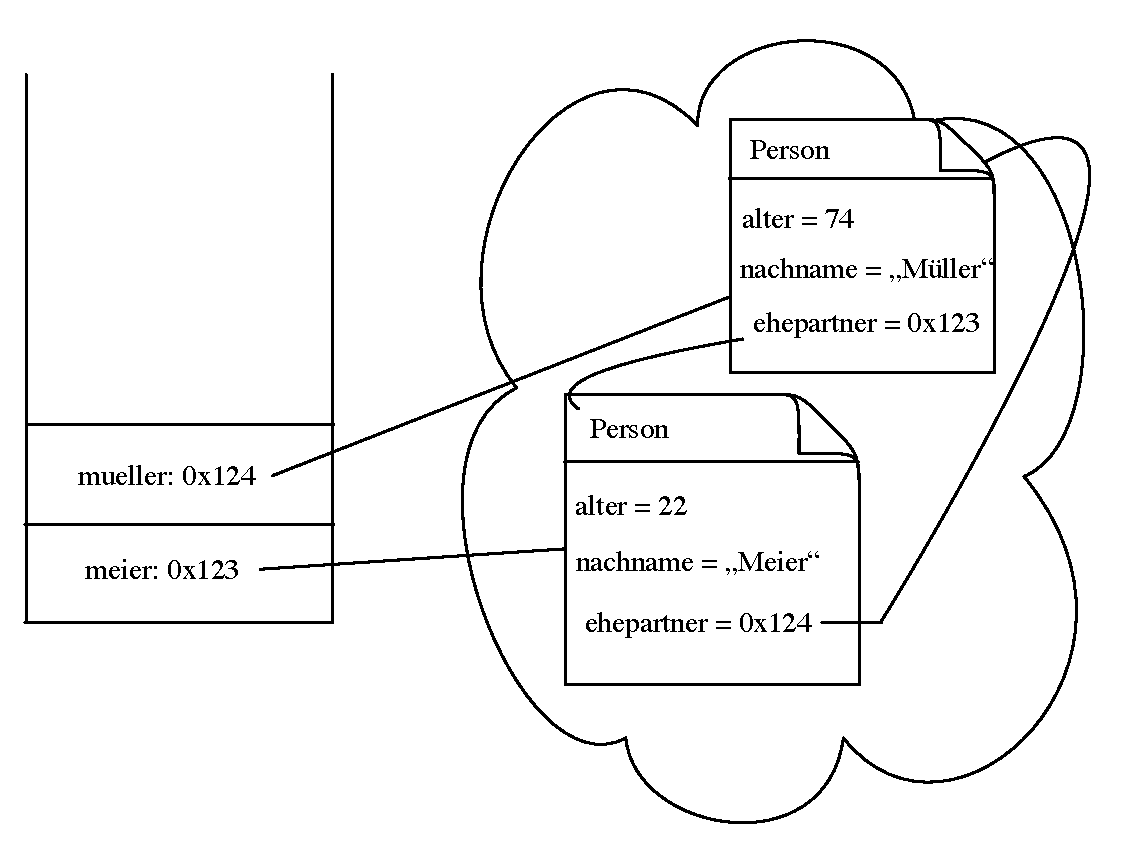
\includegraphics[width=0.8\textwidth]{stackheap_2}
\label{fig:stackheap2}
\caption{Der Stack und Heap nach dem Aufruf der Methode heiraten().}
\end{figure}

Es gilt zu beachten, dass hier die String Literale, die in \texttt{nachname} gespeichert werden, hier vereinfacht wie Instanzvariablen behandelt wurden. In der Realität sind Strings jedoch auch Objekte und somit würde nachname eigentlich auf ein anderes Objekt vom Typ String zeigen, welches dann den Nachnamen darstellt. Ich habe der Anschaulichkeit halber die Strings jedoch wie Instanzvariablen behandelt.

\subsubsection{Garbage Collector}
Ein interessantes Konzept ist das des Garbage Collectors, welches hier nur angeschnitten werden soll. Dieser ist für die Speicherverwaltung auf dem Heap zuständig und sorgt dafür, dass nicht mehr benutzte Objekte aus dem Heap genommen werden, um Speicherplatz zu sparen. Es gibt verschiedene Möglichkeiten, zu bestimmen, welche Objekte wann nicht mehr gebraucht werden, jedoch ist dies ein eigenes Feld für sich und wird eventuell in einer späteren Vorlesung genauer besprochen.

\section{UML}

Die \texttt{Unified Modeling Language} ist eine standardisierte Modellierungssprache, die 1997 aus vielen verschiedenen Modellierungssprachen in der Version 1.0 vereint wurde. Diese Modellierungssprache wird benutzt, um Objekte abstrahiert darzustellen, sodass man ohne die genaue Logik zu verstehen, eine ungefähre Ahnung hat, was ein Programm macht. Das Vereinfachen von komplexeren Abläufen ist also die Grundidee von UML.
Ein Modell ist damit kein exakter Nachbau eines Objektes, sondern eine Vereinfachung, welche das Original beschreibt. Dies bezweckt ein besseres Verständnis des Originals.

Trotz des Teilworts \textit{Language} handelt es sich bei UML um Zeichnungen; diese werden als Diagramme bezeichnet. Es gibt unterschiedliche Arten von Diagrammen, die unterschiedliche Aspekte eines Programms berücksichtigen. Insgesamt gibt es 13 verschiedene Diagrammtypen, die entweder \texttt{Strukturdiagramme} sind, oder aber \texttt{Verhaltensdiagramme}. Strukturdiagramme sind (wer hätte es gedacht) Modelle einer Struktur und somit auch statisch. Hier werden Zusammenhänge beschrieben, was wir im Folgenden anhand der \texttt{Klassendiagramme} zeigen werden. Verhaltensdiagramme erklären die Abläufe eines Programms und sind aus diesem Grund dynamisch. \texttt{Aktivitätsdiagramme} zählen zu den Verhaltensdiagrammen.

\section{Aktivitätsdiagramme}

Aktivitätsdiagramme beschreiben den Ablauf, wie ein Programm funktioniert, besonders die Eigenschaft, dass die Reihenfolge dargestellt wird ist teilweise sehr praktisch, um nachzuvollziehen, was ein Programm macht. Prinzipiell kennt ein Aktivitätsdiagramm nur zwei Arten von Bausteinen. Knoten und Kanten. Knoten sind die Stellen, an denen etwas passiert, und werden deshalb auch als \texttt{Aktivitäten} bezeichnet; Kanten verbinden diese Aktivitäten miteinander. Es gibt zudem noch Startknoten und Endknoten. \underline{Wichtig:} Es ist zwar unüblich, dass mehrere Start- und/oder Endknoten vorkommen, aber dies ist nicht verboten.

Wie der Name es schon impliziert, beginnt eine Prozedur bei einem Startknoten. Man kann sich vorstellen, dass ein \texttt{Token} von dort aus über die Kanten zu den einzelnen Knoten fährt, dort eine Aktion ausgeführt wird und das Token im Anschluss weiterfährt, bis es zu einem Endknoten gelangt.

Wir möchten uns nun angucken, wie ein solches Aktivitätsdiagramm aussieht.

\subsubsection{Beispiel}

\begin{mpost}[mpsettings={input metauml;},use]
Begin.b;
Activity.eat("Esse Etwas");
Branch.enough;
Fork.fork("h", 50);
Activity.read("Lies ein Buch");
Activity.listen("Musik hören", "(im Hintergrund)");
Fork.join("h", 50);
End.e;

leftToRight.top(10)(read, listen);
Group.readListen(read, listen);

leftToRight(30)(b, eat);
topToBottom(20)(eat, enough, fork, readListen, join, e);

drawObjects(b, eat, enough, fork, readListen, join, e);

clink(transition)(b, eat);
clink(transition)(eat, enough);
link(transition)(pathStepX(enough.e, eat.e, 80));
clink(transition)(enough, fork);
clink(transition)(fork, read);
clink(transition)(fork, listen);
clink(transition)(read, join);
clink(transition)(listen, join);
clink(transition)(join, e);

item(iGuard)("[noch hungrig]")(obj.sw = enough.e + (20, 0));
item(iGuard)("[satt]")(obj.nw = enough.s + (0, -4));
  	  
\end{mpost}

Das oben abgebildete Diagramm beinhaltet alle wichtigen Komponenten, die nötig sind, wenn man einen Ablauf beschreibt. Es ist schnell erkenntlich, was dort dargestellt wird. Man isst etwas. Es wird geprüft, ob man satt ist, ist dies nicht der Fall, isst man so lange weiter, bis man satt ist. Im Anschluss liest man ein Buch und \underline{parallel} dazu hört man Musik. Außerdem sieht man hier, wie die Knoten und Kanten aussehen. Wir wollen jetzt etwas genauer auf die verschiedenen Objekte eingehen.

\subsection{Start- und Endknoten}

Es muss für einen Menschen, der sich mit dem Programm, bzw. der Prozedur noch gar nicht auskennt, schnell ersichtlich sein, wo ein Programm beginnt und wann dieses beendet ist. Dazu sind spezielle Knoten wichtig, die unten abgebildet sind. Der ausgefüllte Knoten ist ein Startknoten, der ausgefüllte Knoten mit dem Kreis drum, ist ein Endknoten.\\

\begin{mpost}[mpsettings={input metauml;},use]
Begin.b;
End.e;
leftToRight(20)(b, e);
drawObjects(b, e);
\end{mpost}

\subsection{Aktionen}

Aktionen werden durch Knoten mit einem rechteckigen Kasten und abgerundeten Ecken dargestellt. Darin steht kurz und knapp, welche Aktion bei diesem Knoten ausgeführt wird. Es ist eventuell sinnvoll, sich vorzustellen, dass jede Aktion der Aufruf einer Funktion im Programm ist.\\


\begin{mpost}[mpsettings={input metauml;},use]
Activity.A("Male Aktivitätsdiagramm");
drawObject(A);
\end{mpost}

\subsection{Verzweigungen}
Verzweigungen sind sinnvoll, um ein komplexeres Programm zu schreiben. Im Beispiel oben soll beispielsweise so lange gegessen werden, bis man satt ist. Somit gibt es nach der Aktion essen zwei Möglichkeiten: Weiter essen, oder zur nächsten Aktion springen. Bereits die Fomulierung ähnelt sehr stark einer Schleife aus der Programmierung. 

\begin{lstlisting}
do {
	nimmNahrungAuf();
} while (hungrig());
\end{lstlisting}

Dies entspricht diesem Aktivitätsdiagramm: \\

\begin{mpost}[mpsettings={input metauml;},use]
Begin.b;
Activity.eat("Esse Etwas");
Branch.enough;
End.e;

leftToRight(30)(b, eat);
topToBottom(20)(eat, enough, e);

drawObjects(b, eat, enough,e);

clink(transition)(b, eat);
clink(transition)(eat, enough);
link(transition)(pathStepX(enough.e, eat.e, 80));
clink(transition)(enough, e);

item(iGuard)("[noch hungrig]")(obj.sw = enough.e + (20, 0));
item(iGuard)("[satt]")(obj.nw = enough.s + (0, -4));
\end{mpost}

Nehmen wir nochmal das Token, das über die Kanten zu den verschiedenen Knoten fährt. Dann nimmt dieses Nahrung auf, fährt zu der Verzweigung und es wird geguckt, ob genug Nahrung aufgenommen wird. An den ausgehenden Kanten sieht man, welche der jeweiligen Wege das Token einschlagen wird, da dort (in eckigen Klammern) die Bedingung zum weiterfahren steht. Somit hat es etwas von einem if statement, welches true, oder false zurückgibt. Somit sind sowohl sehr unterschiedliche Wege möglich und im speziellen, wie im Beispiel, Schleifen.
Verzweigungen führen jedoch nicht immer nur verschiedene Kanten in verschiedene Richtungen, sie werden auch genutzt um unterschiedliche Pfade zusammen zu führen. 

\subsection{Gabelungen}

Bei Verzweigungen wird ja das Token nur auf eine der ausgehenden Kantenlinien weitergeleitet. Möchte man jedoch bestimmte Schritte nebeneinander ausführen (Stichwort: Multitasking), so sind \texttt{Gabelungen} nötig. Hier wird das Token kopiert und nimmt jede der möglichen Ausgangskanten. 
Dies sieht dann so aus: \\

\begin{mpost}[mpsettings={input metauml;},use]
Begin.b;
Fork.fork("h", 50);
Activity.read("Lies ein Buch");
Activity.listen("Musik hören");
Fork.join("h", 50);
End.e;

leftToRight.top(10)(read, listen);
Group.readListen(read, listen);

topToBottom(20)(b, fork, readListen, join, e);

drawObjects(b, fork, readListen, join, e);

clink(transition)(b, fork);
clink(transition)(fork, read);
clink(transition)(fork, listen);
clink(transition)(read, join);
clink(transition)(listen, join);
clink(transition)(join, e);
\end{mpost}

Bei diesem Aktivitätsdiagramm wird zur selben Zeit gelesen und Musik gehört. Am Ende, wenn Beides beendet ist, terminiert das Programm. Es ist sehr wichtig zu beachten, dass beim zusammenführen auf die anderen noch laufenden Prozesse gewartet wird. Erst wenn alle Aktionen abgeschlossen sind und bei der Gabelung (die die Kanten wieder zusammen fasst) eintreffen, läuft das Programm weiter.

Nehmen wir als Beispiel den Boxenstopp eines Rennautos: Das Auto fährt in die Boxengasse und ab dem Zeitpunkt wo es hält, werden unterschiedliche Aktionen (parallel) ausgeführt: Die Reifen werden gewechselt, das Rennauto wird betankt, das Visier des Rennfahrers wird eventuell geputzt usw. Der Rennfahrer darf aber erst weiterfahren, wenn alle diese Aktionen abgeschlossen sind, sonst steckt eventuell noch der Tankrüssel im Wagen.

\section{Klassendiagramme}

\texttt{Klassendiagramme} werden dazu benutzt um den Aufbau von Klassen zu beschreiben und die Zusammenhänge zwischen einzelnen Klassen darzustellen. Es ist sehr praktisch objektorientierte Projekte anhand dieser Klassendiagramme zu planen, da man die einzelnen Eigenschaften der Objekte sehr schön darstellen kann und somit einen engen Bezug zur Wirklichkeit hat. Aber bevor wir auf diese Eigenschaften näher eingehen wollen, möchten wir uns erst einmal die Beziehungen zwischen den Klassen ansehen.

\subsection{Assoziation}
\begin{mpost}[mpsettings={input metauml;},use]
Class.A("Klasse A")()();

Class.B("Klasse B")()();

leftToRight(100)(A, B);
drawObjects(A, B);

link(associationUni)(A.e -- B.w);
\end{mpost}\\

Die Verbindungslinie zwischen der \texttt{Klasse A} zu der \texttt{Klasse B} bedeutet, dass \texttt{Klasse A} auf \texttt{Klasse B} zugreifen kann. Die Pfeilrichtung gibt an, welche Klasse auf wen Zugriff hat, es ist auch möglich, dass beiden Klassen aufeinander zugreifen, dann ist an beiden Enden der Verbindungslinie ein Pfeil. Es ist auch möglich die Pfeilspitzen wegzulassen, das ist bei unwichtigen Beziehungen teilweise der Fall.


\subsection{Komposition}
\begin{mpost}[mpsettings={input metauml;},use]
Class.C("Klasse C")()();

Class.D("Klasse D")()();

leftToRight(100)(C, D);
drawObjects(C, D);

link(composition)(C.e -- D.w);
\end{mpost}\\

Hier ist eine \texttt{Komposition} dargestellt. Eine Komposition bedeutet, dass eine Klasse ohne eine andere Klasse nicht auskommt. Die Raute befindet sich an dem Ende der Verbindungslinie, an dem die abhängige Klasse steht. Nehmen wir als Beispiel die Klassen Mensch und Erde. Ein Mensch muss auf der Erde leben, die Erde kann aber auch ohne Menschen auskommen.

\subsection{Vererbung}
\begin{mpost}[mpsettings={input metauml;},use]
Class.E("Klasse E")()();

Class.F("Klasse F")()();

leftToRight(100)(E, F);
drawObjects(E, F);

link(inheritance)(E.e -- F.w);
\end{mpost}\\

Der Vollständigkeit halber soll hier auch einmal die Beziehung im Sinne der Vererbung gezeigt werden. Da Vererbung aber noch nicht in der Vorlesung besprochen wurde, wird hierauf im Weiteren nicht näher eingegangen.

\subsection{Assoziationen verfeinern}

Oben haben wir gesehen, dass man beschreiben kann, ob eine Klasse von einer Anderen abhängig ist. Möchte man jedoch genauer sagen, in welchem Maße diese Abhängigkeit steht, kann man sog. \texttt{Multiplizitäten} angeben. Es gibt \texttt{1:1}, \texttt{1:n} und \texttt{n:n} Beziehungen. Steht keine genauere Angabe an den Verbindunglinien, wird von einer 1:1 Beziehung ausgegangen. Das bedeutet, dass jedes Objekt einer Klasse mit genau einem Objekt der anderen Klasse in Kontakt steht. Eine 1:n Beziehung wird angegeben, wenn ein Objekt einer Klasse mit mehreren Objekten einer anderen Klasse in Kontakt steht. Somit ist auch klar, dass eine n:n Beziehung aussagt, dass Objekte beider Klassen Zugriff auf mehrere Objekte der anderen Klasse haben. Wie bereits beschrieben, muss man 1:1 Beziehungen nicht explizit angeben. Um eine 1:n Beziehung darzustellen, schreibt man ein 0..* an das navigierbare Ende. 0..* liest man wie $n \in N_{0}$.\\

\begin{mpost}[mpsettings={input metauml;},use]
Class.A("Klasse A")()();

Class.B("Klasse B")()();

leftToRight(100)(A, B);
drawObjects(A, B);

link(associationUni)(A.e -- B.w);
item(iAssoc)("0..*")(obj.n  = .8[A.e,B.w]);

\end{mpost}\\

Man kann somit aber auch Ober- und Untergrenzen festlegen, also beispielsweise 2..5 (mindestens 2, aber maximal 5).

\subsection{Klassen beschreiben}

Eine Klasse ist ein Rechteck und hat drei Unterbereiche, welche oben bisher leer gelassen wurden. So gibt es den \texttt{Klassennamen}, darunter befinden sich die \texttt{Eigenschaften} und im letzten Unterbereich befinden sich die \texttt{Methoden}. 
%Um möglichst nah an der Objektorientierung zu sein, kann man den Eigenschaften und Methoden auch eine Sichtbarkeit zuordnen, so schreibt man für \texttt{private} ein - (Minuszeichen), für \texttt{public} ein + (Plus) und für \texttt{protected} ein # (Hash-Zeichen). Ein \texttt{Package} kann man über das \tilde (Tildezeichen) definieren. 

Eigenschaften beschreibt man, indem man den Namen angibt, danach kommt ein Doppelpunkt und zuletzt der Datentyp. Bei den Methoden sieht es fast genau so aus, hier kommt zuerst der Methodenkopf und nach dem Doppelpunkt dann der Rückgabewert. Wie bei Java auch, benutzt man bei Klassendiagrammen \texttt{void}, falls man keinen Wert zurück gibt. Hier ist eine Beispielklasse mit verschiedenen Eigenschaften und einer Methode.\\

\begin{mpost}[mpsettings={input metauml;},use]
Class.Person("Person")
		("-alter: int",
		 "-vorname: String",
		 "-nachname: String",
		 "-alter: int"
		 "-freunde: Person 0..*")
		("+heiraten(partner: Person): void",
		 "+sagHallo(): String");

Person.nw = (0, 0);
drawObject(Person);
\end{mpost}\\

Hier haben wir eine Klasse \texttt{Person} mit den privaten Eigenschaften \texttt{vorname} und \texttt{nachname} vom Typ \texttt{String}, der Eigenschaft \texttt{alter} vom Typ int und eine Liste von \texttt{Personen}, die als \texttt{freunde} bezeichnet werden. Alle diese Eigenschaften sind private, bei dem hier benutzten Programm wird dafür ein Schloss verwendet, jedoch ist es üblicherweise einfach ein - (Minuszeichen).

Zudem besitzt diese Klasse zwei Methoden, die beide \texttt{public} sind. Die Methode \texttt{heiraten()}, die den Rückhabewert void hat (also nichts zurück gibt), nimmt einen Parameter \texttt{partner}, der vom Typ \texttt{Person}, entgegen. Und die Methode \texttt{sagHallo()} gibt einen String zurück.

Man sieht, dass die Klassendiagramme einen guten ersten Eindruck über Klassen geben und man die Logik die hinter den einzelnen Methoden steht, nicht unbedingt verstehen muss.
